\documentclass[12pt, oneside]{article}

\usepackage[letterpaper, scale=0.8, centering]{geometry}
\usepackage{fancyhdr}
\setlength{\parindent}{0em}
\setlength{\parskip}{1em}

\pagestyle{fancy}
\fancyhf{}
\renewcommand{\headrulewidth}{0pt}
\rfoot{{\footnotesize Copyright Daniel Grier / Mia Minnes, 2023, Version \today~(\thepage)}}

\author{CSE105Sp23}

\newcommand{\instructions}{{\bf For all HW assignments:} Weekly homework 
may be done individually or in groups of up to 3 students. 
You may switch HW partners for different HW assignments. 
The lowest HW score will not be included in your overall HW average. 
Please ensure your name(s) and PID(s) are clearly visible on the first page of your homework submission 
and then upload the PDF to Gradescope. If working in a group, submit only one submission per group: 
one partner uploads the submission through their Gradescope account and then adds the other group member(s) 
to the Gradescope submission by selecting their name(s) in the ``Add Group Members" dialog box. 
You will need to re-add your group member(s) every time you resubmit a new version of your assignment.
 Each homework question will be graded either for correctness (including clear and precise explanations and 
 justifications of all answers) or fair effort completeness. You may only collaborate on HW with CSE 105 students 
 in your group; if your group has questions about a HW problem, you may ask in drop-in help hours or post a private 
 post (visible only to the Instructors) on Piazza.

All submitted homework for this class must be typed. 
You can use a word processing editor if you like (Microsoft Word, Open Office, Notepad, Vim, Google Docs, etc.) 
but you might find it useful to take this opportunity to learn LaTeX. 
LaTeX is a markup language used widely in computer science and mathematics. 
The homework assignments are typed using LaTeX and you can use the source files 
as templates for typesetting your solutions.
To generate state diagrams of machines, we recommend using Flap.js
or JFLAP. Photographs of clearly hand-drawn diagrams may also be used. We recommend that you
submit early drafts to Gradescope so that in case of any technical difficulties, at least some of your
work is present. You may update your submission as many times as you'd like up to the deadline.


{\bf Integrity reminders}
\begin{itemize}
\item Problems should be solved together, not divided up between the partners. The homework is
designed to give you practice with the main concepts and techniques of the course, 
while getting to know and learn from your classmates.
\item You may not collaborate on homework with anyone other than your group members.
You may ask questions about the homework in office hours (of the instructor, TAs, and/or tutors) and 
on Piazza (as private notes viewable only to the Instructors).  
You \emph{cannot} use any online resources about the course content other than the class material 
from this quarter -- this is primarily to ensure that we all use consistent notation and
definitions (aligned with the textbook) and also to protect the learning experience you will have when
the `aha' moments of solving the problem authentically happen.
\item Do not share written solutions or partial solutions for homework with 
other students in the class who are not in your group. Doing so would dilute their learning 
experience and detract from their success in the class.
\end{itemize}

}

\newcommand{\gradeCorrect}{({\it Graded for correctness}) }
\newcommand{\gradeCorrectFirst}{\gradeCorrect\footnote{This means your solution 
will be evaluated not only on the correctness of your answers, but on your ability
to present your ideas clearly and logically. You should explain how you 
arrived at your conclusions, using
mathematically sound reasoning. Whether you use formal proof techniques or 
write a more informal argument
for why something is true, your answers should always be well-supported. 
Your goal should be to convince the
reader that your results and methods are sound.} }
\newcommand{\gradeComplete}{({\it Graded for completeness}) }
\newcommand{\gradeCompleteFirst}{\gradeComplete\footnote{This means you will 
get full credit so long as your submission demonstrates honest effort to 
answer the question. You will not be penalized for incorrect answers. 
To demonstrate your honest effort in answering the question, we ask 
that you include your attempt to answer *each* part of the question. 
If you get stuck with your attempt, you can still demonstrate 
your effort by explaining where you got stuck and what 
you did to try to get unstuck.} }

\usepackage{tikz}
\usetikzlibrary{automata,positioning,arrows}

\usepackage{amssymb,amsmath,pifont,amsfonts,comment,enumerate,enumitem}
\usepackage{currfile,xstring,hyperref,tabularx,graphicx,wasysym}
\usepackage[labelformat=empty]{caption}
\usepackage{xcolor}
\usepackage{multicol,multirow,array,listings,tabularx,lastpage,textcomp,booktabs}

\lstnewenvironment{algorithm}[1][] {   
    \lstset{ mathescape=true,
        frame=tB,
        numbers=left, 
        numberstyle=\tiny,
        basicstyle=\rmfamily\scriptsize, 
        keywordstyle=\color{black}\bfseries,
        keywords={,procedure, div, for, to, input, output, return, datatype, function, in, if, else, foreach, while, begin, end, }
        numbers=left,
        xleftmargin=.04\textwidth,
        #1
    }
}
{}

\newcommand\abs[1]{\lvert~#1~\rvert}
\newcommand{\st}{\mid}

\newcommand{\cmark}{\ding{51}}
\newcommand{\xmark}{\ding{55}}
 
\newcommand{\SUBSTRING}{\textsc{Substring}}
\newcommand{\REP}{\textsc{Rep}} 
\title{HW4 : Pushdown Automata and Context-free grammars}
\date{Due: May 2nd at 5pm (no penalty late submission until 8am next morning), via Gradescope}

\begin{document}
\maketitle
\thispagestyle{fancy}

\textbf{In this assignment:}

You will  practice with the definition of pushdown automata and context-free grammars and reason
about regular and context-free languages.

\textit{Resources}: To review the topics you are working with for this assignment, 
see the class material from Week 3 through Week 4. We will post frequently asked questions and 
our answers to them in a pinned Piazza post.

\textit{Reading and extra practice problems}: Sipser Sections 2.1, 2.2. 
Chapter 2 exercises 2.1, 2.2, 2.3, 2.4, 2.5, 2.6, 2.7, 2.9, 2.10, 2.11, 2.12, 2.13, 2.16, 2.17.

\textit{Key Concepts:} Pushdown automata, stack, context-free grammars, derivations, 
context-free languages.

\instructions

You will submit this assignment via Gradescope
(\href{https://www.gradescope.com}{https://www.gradescope.com}) 
in the assignment called ``hw4CSE105Sp23''.

\textbf{Requests from your TAs and tutors}
To help us with grading please 
\begin{itemize}
    \item Start each question on a new page.
    \item Label the start of each solution with {\bf Answer}.
\end{itemize}

\textbf{Assigned questions}


\begin{enumerate} 

\item \textbf{A PDA with multiple possibilities} (22 points): \\
Consider the PDA with input and stack alphabet $\Gamma = \{0,1,2\}$ whose ``unfinished" 
state diagram is given below:

\begin{center}
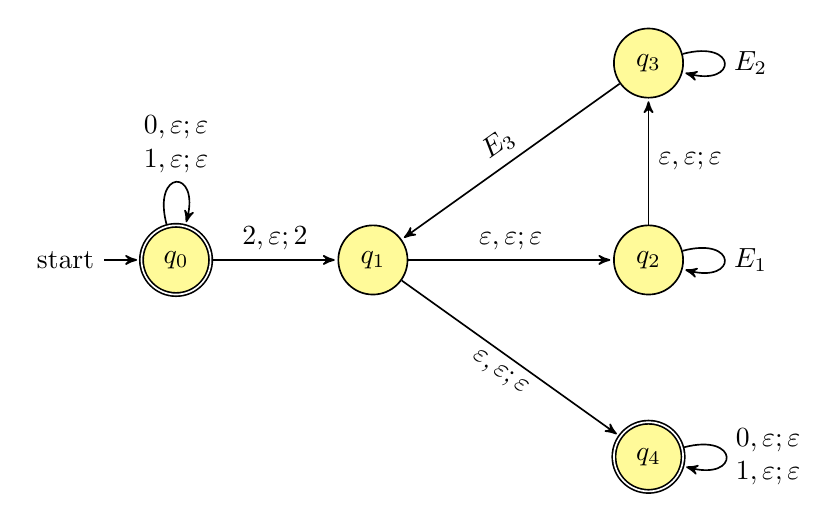
\begin{tikzpicture}[->,>=stealth',shorten >=1pt, auto, node distance=2.5cm, semithick]
  \tikzstyle{every state}=[text=black, fill=yellow!40]

  \node[initial,state, accepting] (q0)      {$q_0$};
  \node[state]         (q1) [right of=q0,  xshift=0cm] {$q_1$};
  \node[state]         (q2) [right of=q1,  xshift=1cm] {$q_2$};
  \node[state]         (q3) [above of=q2] {$q_3$};
  \node[state, accepting]         (q4) [below of=q2] {$q_4$};

  \path (q0) edge [loop above] node[align=left] {$0, \varepsilon; \varepsilon$ \\ $1, \varepsilon; \varepsilon$}  (q0)
  		edge node {$2, \varepsilon; 2$} (q1)
	(q1) 	edge node {$\varepsilon, \varepsilon; \varepsilon$} (q2)
		edge node[below, sloped] {$\varepsilon, \varepsilon; \varepsilon$} (q4)
	(q2) edge [loop right] node {$E_1$} (q2)
		edge [right] node {$\varepsilon, \varepsilon; \varepsilon$} (q3)
	(q3) edge [loop right] node {$E_2$} (q3)
		edge node[sloped] {$E_3$} (q1)
	(q4) edge [loop right] node[align=left] {$0, \varepsilon; \varepsilon$ \\ $1, \varepsilon; \varepsilon$} (q4)
 ;
\end{tikzpicture}
\end{center}

There are three labels ($E_1$, $E_2$, and $E_3$) on the edges that are unspecified. 
To be precise, each $E_i$ is of the form ``$x,y; z$'' where $x, y, z \in \Gamma_{\varepsilon}$ 
(recall $\Gamma_{\varepsilon} = \Gamma \cup \{\varepsilon\}$).

\begin{enumerate}
    \item\gradeCorrectFirst Prove that (no matter how the labels $E_1, E_2, E_3$ are specified), 
    the language recognized by this 
    PDA is infinite. A complete solution will include a precise
    description of an infinite collection of strings each 
    of which is accepted by the PDA, with 
    a precise and
    clear description of the accepting computation of the PDA on 
    each of these strings.

    \item\gradeCompleteFirst Prove/Disprove: Over all the possible choices for the labels $E_1, E_2, E_3$, 
    this PDA can only recognize finitely many languages. Justify your solution by referring back to the 
    relevant definitions.

    \item\gradeCorrect Recall that for $L \subseteq \Sigma^*$ with $\Sigma = \{0,1\}$, we define
    \begin{align*}
    \REP(L) &:= \{ w \in \Gamma^* \mid \text{between every pair of successive $2$'s in $w$ is a string in $L$}\}\\
    &\phantom{:}=\{w \in \Gamma^* \mid \text{for all } v \in \Sigma^* \text{ if } 2v2 \in \SUBSTRING(\{w\})  \text{, then } v \in L\} 
    \end{align*}
    where for all languages $K \subseteq \Gamma^*$ we let
    \[
    \SUBSTRING(K) := \{ w \in \Gamma^* \mid \text{there exist } a,b \in \Gamma^* \text{ such that } awb \in K\}.
    \]

    Determine how to set the labels $E_1, E_2, E_3$ so that the language of the PDA is 
    \[
    \REP(\{0^n1^m \mid n \ge 0, m \ge 0\})
    \]
    In addition to specifying each $E_i$, a complete justification 
    will include a precise description of why this choice of the $E_i$'s
    means that the PDA recognizes the language indicated.

    \item\gradeCorrect Determine how to set the labels $E_1, E_2, E_3$ so that the language of the PDA is 
    \[
    \REP(\{0^n1^n \mid n \ge 0\})
    \]
    In addition to specifying each $E_i$, a complete justification 
    will include a precise description of why this choice of the $E_i$'s
    means that the PDA recognizes the language indicated.
\end{enumerate}

\item \textbf{Grammar practice} (12 points): \\
For each of the languages listed below, 
define a context-free grammar 
$G = (V, \Sigma, R, S)$ that generates the 
language. Instead of formally justifying
your grammar, illustrate it by giving 
{\bf two examples} 
of strings in the language 
and their derivations using your grammar
and {\bf one example} of a string not
in the language with an explanation
of why it cannot appear 
on the right side of any derivation 
in your grammar. Choose your
examples so they are different enough 
to illustrate the role of 
as many of the variables 
in your grammar as possible.

\begin{enumerate}
    \item\gradeCorrect $\REP(\{0^n1^n \mid n \ge 0\})$

    \item\gradeCorrect $\{1^n = 1^a + 1^b \in \{1,=,+\}^* \mid a,b,n \ge 1 \text{ such that } a + b = n \}$
\end{enumerate}

\item \textbf{Substrings and regularity} (16 points): \\
For this problem, we fix the 
alphabet $\Gamma = \{0,1,2\}$. Recall the 
definition of the function $\SUBSTRING$ from 
Problem 1.
\begin{enumerate}
\item\gradeCorrect Prove that $\SUBSTRING(\{ 0^n 1^n \mid n \ge 0\})$ is regular.
A complete 
solution will include a 
precise definition of a DFA, NFA, or regular 
expression that recognizes or describes it, along 
with a brief justification
of your construction by explaining the role each 
state plays in the machine
and referring back to relevant definitions.
\item\gradeCorrect Prove that 
$\SUBSTRING(\{ 0^n 1^n 2^n \mid n \ge 0\})$
is not regular.
\item\gradeComplete Is  $\SUBSTRING(\{ 0^n 1^n 2^n \mid n \ge 0\})$
context-free?
Informally justify your answer, referring 
to class discussions and/or the textbook.

\end{enumerate}
\end{enumerate}

\end{document}